Penelitian dimulai dengan pembuatan model senar yang ideal, yaitu sebuah senar homogen dengan kedua ujung terikat. Senar dimodelkan memiliki panjang 20 cm seperti yang biasa dipasang pada \textit{bundengan}, memiliki densitas linear $\mu_s=0,0005$ kg/m seperti densitas linear senar badminton, serta diregangkan oleh sebuah tegangan $T=20$ N. Setelah model senar berhasil dibangun, selanjutnya dilakukan validasi apakah model tersebut sudah sesuai dengan teori. Validasi dilakukan dengan melakukan simulasi pemetikan senar, yaitu memberi perpindahan sebesar 0,5 cm kebawah pada bagian tengah senar. Kemudian dilakukan pengamatan terhadap mode getar dan spektrum frekuensi dari senar tanpa \bandulan yang dipetik di tengah. Gambar \ref{fig:modegetarTanpaBandul} memperlihatkan setiap mode getar dari senar yang dipetik di tengah tanpa \textit{bandulan}, sedangkan Gambar \ref{fig:responwaktuTanpaBandul} memperlihatkan bagaimana senar merespon petikan untuk setiap posisi senar dan setiap waktu. Dari grafik mode getar dan respon waktu tersebut dapat dikonfirmasi bahwa model senar yang dibuat sudah berperilaku seperti senar yang ideal \cite{bukuFletcher}. \par 
\begin{figure}[t!]
    \centering
    \subfigure[]{\label{fig:modegetarTanpaBandul}\includegraphics[width=13 cm]{Gambar/modeGetarTanpaBandul.jpg}} 
    \hspace{1 cm}
    \subfigure[]{\label{fig:responwaktuTanpaBandul}\includegraphics[width=12 cm]{Gambar/spektrumFrekTanpaBandul.jpg}}
    \caption{(a) Mode getar dan (b) spektrum frekuensi dari senar \bundengan tanpa \bandulan yang dipetik pada bagian tengah senar \cite{paperGetaranBandulan}.}
    \label{fig:senarTanpaBandulan}
\end{figure}
Pengamatan pertama dilakukan dengan memasang satu buah \bandulan pada jarak 6 cm dari salah satu ujungnya. Massa \bandulan $m_b$ pada awalnya diatur bernilai 0,5 kali massa senar $m_s$, kemudian diatur menjadi 1000 kali massa senar. Simulasi yang dilakukan sama seperti memvalidasi perilaku senar tanpa \textit{bandulan}, yakni dengan memberi perpindahan 0,5 cm kebawah pada bagian tengah senar. \par 

Perkembangan besar yang telah diberikan Guido dalam pendidikan musik adalah terciptanya sistem di mana notasi rentang nada musik dijelaskan dalam enam segmen not yang saling terkait.
\begin{enumerate}
    \item Posisi \\
    Penempatan sebuah objek memiliki pengaruh yang sangat besar terhadap informasi mengenai suatu hal. Hal ini karena susunan spasial adalah sesuatu yang pertama kali dibaca oleh otak manusia ketika melihat suatu tampilan yang kompleks. Skema penempatan posisi terbaik adalah meletakkan setiap objek grafis pada posisi unik, sehingga semuanya dapat dilihat dengan jelas tanpa adanya tumpang-tindih antar objek. Penentuan posisi objek grafis juga dipengaruhi oleh variabel yang hendak direpresentasikan. Pemusatan data, distribusi statistik, serta tren pada data dipengaruhi oleh variabel apa yang direpresentasikan. Skala digunakan untuk mengorganisir ruang tampilan dan untuk menghadirkan struktur nilai yang representatif. Yang pertama adalah skala linear, yaitu dengan memetakan setiap data pada rentang nilai tertentu. Yang kedua adalah skala logaritmik, di mana skala ini digunakan untuk memetakan data dengan peningkatan nilai yang eksponensial supaya didapatkan rentang nilai yang lebih mudah diamati.
    \item Bentuk \\
    Bentuk adalah konstruksi yang terdiri dari titik, garis, area, dan volume. Perbedaan konstruksi tersebut dapat dijadikan sebagai penanda dua hal yang berbeda ketika menampilkan data. Bentuk-bentuk umum yang digunakan diantaranya adalah lingkaran, persegi, segitiga, bintang, maupun tanda silang. Pertimbangan paling penting dalam pemilihan bentuk adalah seberapa jelas setiap bentuk dapat dibedakan. Hal ini karena pandangan manusia akan sulit untuk mengobservasi sesuatu yang terlihat mirip. Pada Gambar \ref{fig:clef-macammacam} diperlihatkan tiga bentuk \textit{clef} yang dapat dibedakan dengan jelas. \begin{figure}[t!]
        \centering
        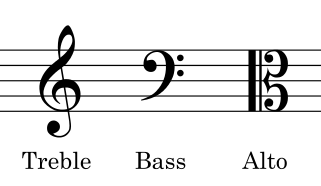
\includegraphics[width=6cm]{Gambar/clef-macam-macam.jpg}
        \caption{Contoh penggunaan bentuk berbeda dalam notasi musik \cite{bukuTeoriMusik}.}
        \label{fig:clef-macammacam}
    \end{figure} Bentuk yang mudah dibedakan ini tentu akan meningkatkan tingkat keefektifan suatu sistem visual.
    \item Ukuran (Panjang, Luas, dan Volume) \\
    Variabel visual yang ketiga adalah ukuran. Seberapa besar dan kecilnya objek visual ditentukan dengan ukuran. Perbedaan yang dapat terlihat dalam ruang ini mampu merepresentasikan nilai tertentu. Peningkatan ukuran dapat dijadikan penggambaran peningkatan nilai variabel yang lebih mudah diproses persepsi manusia. 
    \item Kecerahan \\
    Kecerahan atau luminansi adalah tingkat hitam–putih suatu objek visual. Kecerahan dapat digunakan untuk dijadikan pembeda untuk beberapa nilai data. Meskipun demikian, kecerahan tidak dapat digunakan sebagai penanda untuk setiap data pada rentang yang lebar secara terpisah. Hal ini karena persepsi manusia tidak dapat membedakan dengan detil tingkat kecerahan suatu objek untuk kemudian diasosiasikan dengan nilai tertentu. Dengan kata lain, kecerahan hanya efektif digunakan untuk merepresentasikan dua nilai yang sangat kontras perbedaannya.  
    \item Warna \\
    Kecerahan menyatakan seberapa hitam atau seberapa putihnya objek visual, namun sebenarnya yang dinyatakan oleh kecerahan bukanlah warna. Warna dapat didefinisikan dengan dua parameter, yaitu \textit{hue} dan saturasi. Pada Gambar \ref{fig:macam-warna} diperlihatkan pilihan warna dari Microsoft dengan \textit{hue} dinyatakan pada sumbu mendatar dan saturasi pada sumbu tegak. \textit{Hue} menyatakan sesuatu yang kita anggap sebagai warna, yaitu panjang gelombang dari cahaya tampak. Sedangkan saturasi adalah tingkat \textit{hue} relatif terhadap keabu-abuan. Saturasi juga memperlihatkan kemurnian suatu warna yang ditampilkan. Pada penggunaan warna untuk representasi kumpulan informasi, diperlukan pemetaan data pada masing-masing warna. Digunakannya warna sebagai salah satu variabel visual dapat diamati pada Tabel \ref{tab:prosidingDirektivitas}, di mana rentang nilai TTB dinyatakan dalam rentang warna merah sampai biru. \begin{figure}[t!]
        \centering
        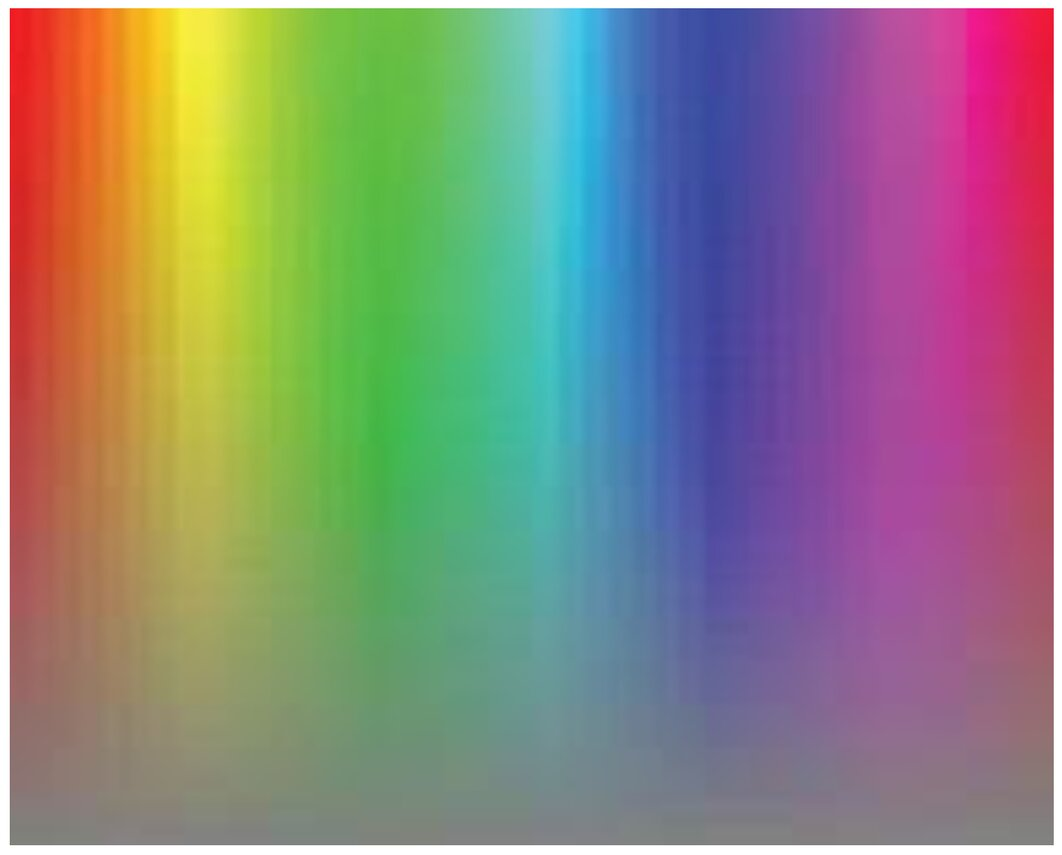
\includegraphics[width=6cm]{Gambar/macam-warna.jpg}
        \caption{\textit{Hue} dan saturasi pada pilihan warna Microsoft \cite{buku_visual}.}
        \label{fig:macam-warna}
    \end{figure}
    \item Orientasi \\
    Orientasi adalah arah dari sebuah objek visual. Variabel visual ini menyatakan bagaimana sebuah bentuk diputar sehubung dengan informasi yang hendak disampaikan. Perbedaan orientasi tidak selalu dapat digunakan pada semua bentuk objek visual. Penerapan orientasi yang paling baik adalah pada bentuk yang hanya memiliki satu sumbu simetri, seperti segitiga sama kaki. Hal ini karena perbedaan orientasi pada bentuk dengan banyak sumbu simetri tidak terlalu kontras, sehingga persepsi manusia sulit untuk memindai informasi yang hendak disampaikan.
    \item Tekstur \\
    Variabel visual yang ketujuh adalah tekstur. Tekstur dapat dikatakan sebagai kombinasi berbagai variabel visual, seperti bentuk, warna, dan orientasi. Garis putus-putus dan titik-titik yang membentuk garis dapat dikategorikan sebagai tekstur. Penggunaan tekstur biasanya diasosiasikan dengan area atau permukaan tertentu. Pada bidang 3D, tekstur dapat berupa perbedaan geometri seperti ketinggian pada permukaan.
    \item Gerakan \\
    Variabel visual yang terakhir adalah gerakan. Penerapan umum dari gerakan adalah dengan memvariasikan kecepatan dari perubahan setiap objek visual. Perubahan yang dimaksud dapat berupa perubahan posisi, berkedip, warna, ataupun tingkat gelap–terang. Gerakan dapat berguna untuk menyampaikan informasi karena pandangan manusia akan mengamati perubahan perilaku dari setiap objek visual, tidak hanya perilaku yang mirip, namun perilaku yang bertentangan juga dapat berupa sebuah informasi. 
\end{enumerate}
\begin{table}[b!]
    \begin{center}
        \caption{Faktor-faktor penentu pemilihan ukuran sampel \cite{bukuUlrich}.}
    \end{center}
    \begin{tabular}{m{7cm} m{7cm}}
        \hline
        \textbf{Faktor pendukung pemilihan sampel yang sedikit} & \textbf{Faktor pendukung pemilihan sampel yang banyak}\\
        \hline
        \begin{itemize}
            \item Pengujian dilakukan pada awal proses pengembangan
            \item Pengujian dilakukan untuk mendapatkan data kualitatif
            \item Pencarian sampel dan pelaksanaan survei menghabiskan banyak waktu dan biaya
            \item Biaya untuk pengembangan dan produksi tergolong rendah
        \end{itemize} & \begin{itemize}
            \item Pengujian dilakukan setelah proses pengembangan
            \item Pengujian dilakukan dengan tujuan mengetahui permintaan secara kuantitatif
            \item Pencarian sampel dan pelaksanaan survei relatif cepat dan murah.
            \item Biaya untuk pengembangan dan produksi tergolong tinggi
        \end{itemize} \\
        \hline
    \end{tabular}
    \label{tab:ukuran-sampel}
\end{table}

\begin{figure}[b!]
    \centering
    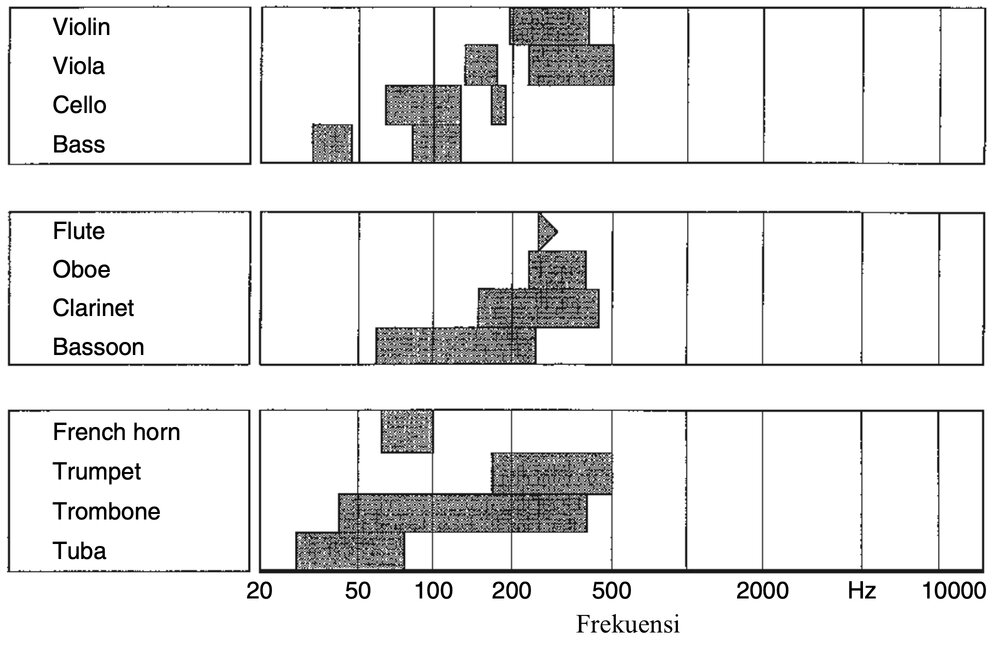
\includegraphics[width= 13.3 cm]{Gambar/frek-region-omni.jpg}
    \caption{Daerah frekuensi pada bunyi instrumen musik orkestra yang bersifat omnidireksional \cite{meyer}.}
    \label{fig:reg-frek-orkestra}
\end{figure}


\begin{enumerate}
    \item \textbf{"Apa?" bukan "Bagaimana?"}
    \begin{enumerate}
        \item \textbf{Pernyataan:} "Saya ingin iPhone saya dapat mengatur termostat."
        \item \textbf{Kebutuhan –– Benar:} Termostat dapat diatur dari jarak jauh.
        \item \textbf{Kebutuhan –– Salah:} Termostat hadir dengan piranti lunak pada iPhone.
    \end{enumerate}
    \item \textbf{Spesifik}
    \begin{enumerate}
        \item \textbf{Pernyataan:} "Saya memiliki sistem pemanas dan pendingin yang berbeda."
        \item \textbf{Kebutuhan –– Benar:} Termostat dapat mengatur sistem pemanas dan pendingin yang terpisah.
        \item \textbf{Kebutuhan –– Salah:} Termostat ini harus serbaguna.
    \end{enumerate}
\end{enumerate}




%---- bab 4

Pada bagian ini:
\begin{enumerate}[label=\alph*)]
\item Uraikan secara rinci spesifikasi dan jangkauan kemampuan alat yang digunakan. Alat
bisa berupa perangkat keras (\textit{hardware}) maupun perangkat lunak (\textit{software}).
\item Jika penelitian melibatkan penggunaan bahan-bahan (kimiawi, fisik, dll.), uraikan
spesifikasi bahan yang digunakan.
\item Jika penelitian bersifat empirik, gambarkan rancangan sistem alat untuk penelitian.
\end{enumerate}



\section{Tata Laksana Penelitian}
 Uraikan rangkaian logis penyelesaian masalah menurut tahap-tahap
analisis yang dipaparkan dalam bagian \textbf{Dasar Teori}, yaitu berupa langkah-langkah
kerja dan/atau algoritma penelitian.


\section{Rencana Analisis Hasil}
Kemukakan bagaimana, menurut rencana, hasil-hasil yang akan
diperoleh dari penelitian akan diolah. Cara bagaimana pengolahan ini akan dilakukan
sudah tentu disesuaikan/dikaitkan dengan tujuan penelitian. Secara umum, pengolahan bisa
dilakukan melalui proses:
\begin{enumerate}[label=\alph*)]
\item \textbf{Perangkuman} hasil penelitian dalam format tabel, gambar, statistik (rata-rata,
koefisien korelasi, dlsb.), atau dalam bentuk besaran khusus tertentu sesuai dengan
parameter atau variabel yang dilibatkan dalam penelitian.
\item Pengujian \textbf{perbedaan} statistik (rata-rata, korelasi, dlsb) variabel penelitian.
\item Pengujian \textbf{keterkaitan} (korelasi) statistik variabel penelitian.
\item Pengolahan lain yang relevan dengan tujuan penelitian.
\end{enumerate}